% SPDX-License-Identifier: CC-BY-4.0
%
% Copyright (c) 2023 Nelson Vieira
%
% @author Nelson Vieira <nelson0.vieira@gmail.com>
% @license CC-BY-4.0 <https://creativecommons.org/licenses/by/4.0/legalcode.txt>
% \documentclass[sigconf,natbib=false]{acmart}
\documentclass[manuscript,natbib=false]{acmart}

% \usepackage{amsmath,amssymb,amsfonts}
% \usepackage{algorithmic}
% \usepackage{graphicx}
% \usepackage{textcomp}
% \usepackage{xcolor,colortbl}

%% \BibTeX command to typeset BibTeX logo in the docs
% \AtBeginDocument{%
%   \providecommand\BibTeX{{%
%     Bib\TeX}}}

%% Rights management information.
%% ! Change after completing the rights form.
\setcopyright{none}
% \copyrightyear{2023}
% \acmYear{2023}
% \acmDOI{XXXXXXX.XXXXXXX}

% \acmConference[GoodIT 2023]{ACM 3rd International Conference on Information
% Technology for Social Good}{September 06--08, 2023}{Lisbon, Lisbon}

%% Might change this if a submission ID is received after rights form.
%%\acmSubmissionID{123-A56-BU3}

\RequirePackage[
    datamodel=acmdatamodel,
    style=acmnumeric,
]{biblatex}

\addbibresource{assets/references.bib}

\begin{document}

%% The "title" command has an optional parameter,
%% allowing the author to define a "short title" to be used in page headers.
\title{Empowering Users' Privacy Rights in the Internet of Things}

%% Of note is the shared affiliation of the first two authors, and the
%% "authornote" and "authornotemark" commands
%% used to denote shared contribution to the research.
\author{Nelson Vieira}
\authornote{Work done as part of master's thesis.}
\email{2080511@student.uma.pt}
\orcid{0009-0008-6055-2954}
\affiliation{%
    \institution{University of Madeira}
    \department{Faculty of Exact Sciences and Engineering}
    \streetaddress{Campus Universitário da Penteada}
    \city{Funchal}
    \state{Madeira}
    \country{Portugal}
    \postcode{9020-105}
}

\author{Mary Barreto}
\authornote{Coordinator of this work.}
\email{mary.barreto@staff.uma.pt}
\orcid{0000-0002-9619-4254}
\affiliation{%
    \institution{University of Madeira}
    \department{Faculty of Exact Sciences and Engineering}
    \streetaddress{Campus Universitário da Penteada}
    \city{Funchal}
    \state{Madeira}
    \country{Portugal}
    \postcode{9020-105}
}

\renewcommand{\shortauthors}{Vieira and Barreto}

\begin{abstract}
    Since the advent of ubiquitous computing, the idea of millions of connected
    devices controlling every aspect of our lives has become a reality. These
    devices are known as Internet of Things (IoT) devices. Today, we have smart
    homes, smart cities, smart wearables, smart vehicles, and many more items
    that connect through a variety of networks and devices. New methods of
    gathering and processing personal data from users and non-users are
    made possible by these devices. The majority of end users have little
    or no control over the data that these systems are gathering about them.
    This work adopts an holistic approach to the issue by first conducting a
    literature review, then a survey to find out more about the public's
    general knowledge, and subsequently, utilizing the information gathered,
    a system is proposed that provides users information about the nearby
    devices and how to protect the data they do not want to share with these
    devices. This system is capable of detecting what kind of devices are
    nearby, what kind of data is being shared, and how close the devices
    are to the user.
    \end{abstract}

%% Generated by the tool at http://dl.acm.org/ccs.cfm.
\begin{CCSXML}
    <ccs2012>
        <concept>
            <concept_id>10002978.10003029.10011150</concept_id>
            <concept_desc>Security and privacy~Privacy protections</concept_desc>
            <concept_significance>500</concept_significance>
        </concept>
        <concept>
            <concept_id>10002978.10003029.10003032</concept_id>
            <concept_desc>Security and privacy~Social aspects of security and privacy</concept_desc>
            <concept_significance>500</concept_significance>
        </concept>
    </ccs2012>
\end{CCSXML}

\ccsdesc[500]{Security and privacy~Privacy protections}
\ccsdesc[500]{Security and privacy~Social aspects of security and privacy}

\maketitle

\keywords{privacy, Internet of Things, ubiquitous computing, privacy assistant}

% \begin{teaserfigure}
%     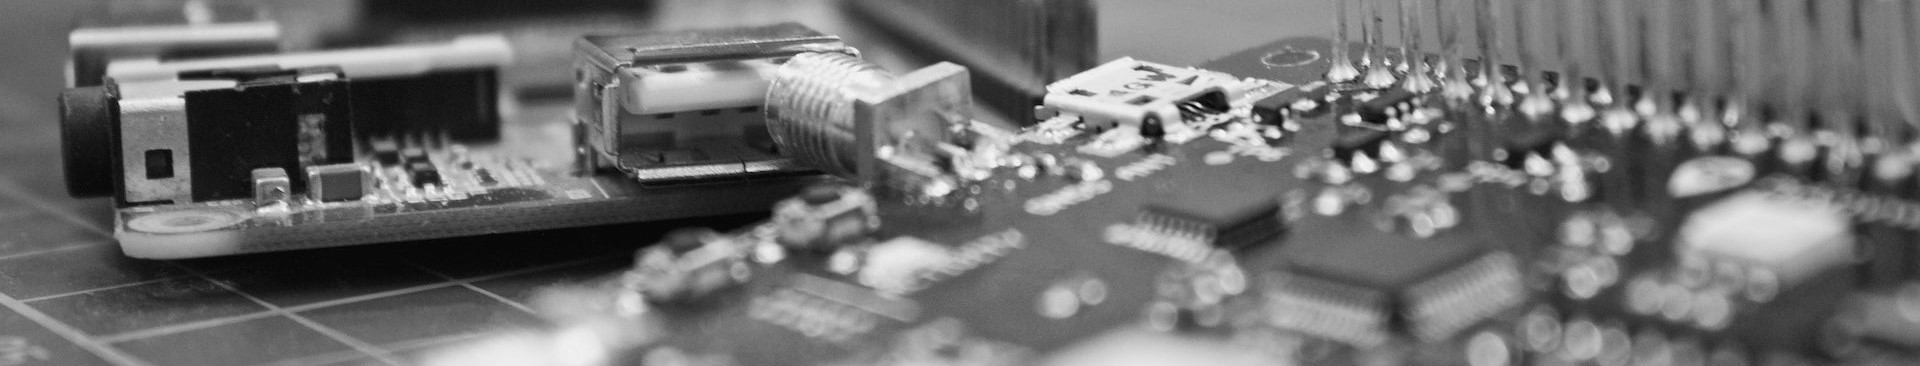
\includegraphics[width=\textwidth]{assets/teaser.jpg}
%     \caption{Internet of Things components.}
%     \Description{Components commonly used in the creation of IoT systems.}
%     \label{fig:teaser}
% \end{teaserfigure}

% \received{1 July 2023}
% \received[revised]{12 March 2009}
% \received[accepted]{5 June 2009}

\section{Introduction}

Privacy as we know it is a somewhat recent concept \cite{vincent2016privacy, moore2017privacy},
before the digital age there was barely any notion of privacy for most
people. Long seen as a luxury, privacy
is still usually regarded as a good to have rather than an essential
requirement, even though it is acknowledged as a human right, as present
in article 12 of the Universal Declaration of Human Rights \cite{RooseveltUniversal}:
``No one shall be subjected to arbitrary interference with his privacy,
family, home or correspondence, nor to attacks upon his honour and reputation.
Everyone has the right to the protection of the law against such interference
or attacks''. Since handling sensitive information requires discretion, privacy
can be defined \cite{InternationalWhat, SpiekermannEngineering}
as the right to control how it is gathered, stored, and used. As a result,
businesses must be upfront and honest about the types of data they intend to
collect, why they need it, and where and with whom they intend to share it.
Users ought to be able to manage how their information is shared.

This definition can cause some confusion with the idea of security \cite{HIVDifference}
and although privacy and security are interconnected, security involves
measures taken to safeguard data from risk, threat or danger, it frequently
alludes to safety. It is the practice of keeping users' personal information
and data safe and preventing unauthorized access to it. The primary contrast
between privacy and security is that the former deals with personal information
to individuals and how they want their data used and maintained, whilst
the latter deals with its protection from possible threats. Security can
exist without privacy, but the opposite is not true.

The previous few years have seen an increase in concerns about online privacy \cite{emami2019exploring, park2022personal, zhang2022peer},
particularly in the wake of the cyberattacks by the decentralized hacker
group Anonymous, WikiLeaks, and Snowden's release of top-secret papers
from the US National Security Agency. When searching for terms like "privacy,"
"online privacy," or "digital privacy" in Google Scholar, ACM Digital Library,
or Science Direct, it can be seen that the number of documents have increased.

The term \textit{Internet of Things} initially originated in the 1990s, and it is
possibly related to Mark Weiser's work on ubiquitous computing \cite{weiser1991computer}
and the proliferation
of devices of all sizes that connect with one another to do various activities,
making Weiser's dream a reality. The term \textit{Internet of Things} was coined in
1999 by British technology pioneer Kevin Ashton \cite{KevinThat}, executive director of the
Auto-ID Center at Massachusetts Institute of Technology (MIT), to describe
a system in which devices with sensors may be connected to the internet.
While making a presentation for Procter \& Gamble, Ashton coined the phrase
to emphasize the need of connecting Radio-Frequency Identification (RFID) tags.

These devices are employed in a variety of applications, for instance at home \cite{marikyan2019systematic}
with thermostats, refrigerators, microwaves, and so on, to
smart vehicles \cite{arena2020overview}, the educational system \cite{al2020survey},
our clothing and watches \cite{niknejad2020comprehensive}, and even
outer space \cite{AkyildizInternet}. IoT resources can include IoT equipment (such as smart home
assistants and autonomous cars), IoT services (such as video analytics
services linked to smart cameras and indoor location monitoring systems),
or IoT apps that track and use information about us. The term "Internet of
Things" refers to scenarios in which a variety of objects, gadgets, sensors,
and everyday items are linked to the internet and have computational capabilities.

% Although the term \textit{Internet of Things} is relatively new, the concept
% of utilizing computers and networks to manage and monitor objects is not.
% The first commonplace object to be connected to the internet was a Coke
% machine at Carnegie Mellon University's Computer Science Department \cite{EverhartInteresting}. The
% 1982 system broadcast the status of each row of the vending machine on
% the network so that it could be accessed using a terminal and the Name/Finger protocol.
% Remotely observing the out of stock lights on the pushing buttons of
% the vending machine. At the Interop Internet Networking exhibition in
% 1990, John Romkey's toaster \cite{RomkeyToast} that could be switched on and off through
% the internet was displayed.

The Internet of Things can be defined as: ``An open and comprehensive network
of intelligent objects that have the capacity to auto-organize, share information,
data and resources, reacting and acting in face of situations and changes
in the environment'' \cite{madakam2015internet}.

IoT is one of the fastest growing technologies \cite{MohammadState}, it
is predicted that it will grow into the trillions of devices by 2030 \cite{SarawiInternet},
and with this expansion new security vulnerabilities and data gathering
dangers appear, the lack of security in these devices makes them ideal targets
for privacy violations and inadequate customer disclosure of device capabilities
and data practices aggravates privacy and security issues.

Privacy in IoT systems in not seen as a crucial factor in development \cite{alhirabi2021security}.
Specific standards for privacy options have been imposed by data privacy
regulations including the General Data Protection Regulation (GDPR) and
California Consumer Privacy Act (CCPA), but even these regulations have
been criticized \cite{peloquin2020disruptive, gladis2022weaponizing, gentile2022deficient, green2022flaws, byun2019privacy}.

\section{State of the Art}

\par
This section provides an overview of the recent literature with the themes
that were found to be more relevant for this work.

\subsection{Privacy Paradox}

The use of a variety of digital devices have numerous advantages, but they
also bring with them the ubiquity of data capturing equipment, therefore,
it is understandable why the majority of online users have serious concerns
about the privacy of their personal data. However, the opinions expressed
are starkly at odds with the reality, according to Thomson et al. \cite{DarrenState}
report on the state of privacy, that just one in four European users read
the terms and conditions in their entirety prior to making an online purchase
or subscribing to a service, 59\% admitted to only quickly scanning the
terms and conditions before completing a purchase, while 14\% admitted to
never reading them at all, 30\% of the respondents would even swap their
email address to win a reward, or entry into a raffle, while 17\% would do
so to get an app and 30\% would do it for money.

This is what is called a privacy paradox, there have been multiple papers
written on this subject \cite{solove2021myth, WilliamsPrivacy, lee2021investigating, goad2021privacy, gerber2018explaining},
some papers attempt a theoretical explanation while others attempt an empirical
one. There has been very different interpretations or explanations of this
paradox, a few papers \cite{wilson2012unpacking, warshaw2015can, lee2015privacy}
apply the theoretical concept of the \textit{homo economicus} \cite{zak2008moral},
which is the representation of people as beings who constantly act in a
way that is logical and self-interested, not worrying about morality or
ethics, and who do so to the best of their ability, to the context of privacy.
Different cognitive biases and heuristics can influence how consumers make
decisions, according to several studies on consumer choice behavior \cite{acquisti2007can, knijnenburg2013dimensionality, wakefield2013influence, flender2012type}.
According to several articles \cite{dienlin2015privacy, baek2014solving},
this paradox might be explained by the fact that some people have genuinely
experienced online privacy assaults and that most privacy views are therefore
based on heuristics or secondhand accounts. Taddicken's study \cite{taddicken2014privacy}
argues that peer pressure is the reason people have this contradictory behavior,
Norberg et al. \cite{norberg2007privacy} explains this paradox by suggesting
that while perceived risk affects reported attitudes and behavioral intentions,
trust has a direct impact on privacy behavior, while others \cite{flender2012type, kokolakis2017privacy}
rely on quantum theory. Brandimarte et al. \cite{brandimarte2013misplaced}
have explored the idea that when it comes to their data privacy, users have
an \textit{illusion of control}.

This paradox has been proven to be vitiated by a number of empirical studies \cite{dienlin2015privacy, xie2019consumers, SCHWAIG20131, sannon2018privacy},
online privacy practices are founded on separate privacy mindsets and so
they are not inherently paradoxical.

\subsection{Privacy in IoT: Approaches}

There have been a number of systematic literature reviews (SLR) \cite{Gupta2022Privacy, Kuhtreiber2022survey, sicari2015security, LinSurvey}
and systematic mapping reviews \cite{porras2018security, ahmed2019aspects}
done to study privacy and security issues in IoT.

Based on Ziegeldorf's \cite{ziegeldorf2014privacy} analysis of the literature,
the following are the most prominent privacy concerns in IoT:

\begin{enumerate}
    \item
    The most prominent concern is \textit{identification}, which binds an
    identifier, such as a name and location, with an individual's identity,
    this also enables and aggravates other threats;
    \item
    \textit{Localization and tracking} is the threat of detecting an individual's
    locations through numerous techniques, such as GPS, internet traffic,
    or smartphone location. This threat requires \textit{identification}
    of some kind;
    \item
    In e-commerce, \textit{profiling} is often used for personalization.
    Organizations collect information about individuals in order to deduce
    their interests via association with other profiles and data sources.
    \item
    \textit{Interaction and presentation} allude to the sharing of private
    information with an unintended audience while doing so through a public
    medium. IoT applications often need extensive user interaction, it is
    expected that users of these systems will obtain information via smart
    devices in their immediate surroundings and that users will interface
    with systems in creative, natural ways. However, many of those modes
    of communication and presentation are already available to the broader
    public, making them apparent to anybody around. When personal information
    is transferred between a system and its user, privacy is breached.
    \item
    \textit{Lifecycle transitions} occur when an IoT device is sold, utilized
    by its owner and eventually disposed of. There may be an expectation
    that the object deletes all information, yet smart devices frequently
    keep massive volumes of data about their own past throughout their entire
    existence. This might contain personal images and videos, which are
    not always erased following ownership transfer.
    \item
    \textit{Inventory attacks} involve unauthorized entry and the acquisition
    of information about the presence and characteristics of personal things.
    Malicious users might use inventory data to profile the property and
    break in.
    \item
    \textit{Linkage} is the process of connecting disparate systems, when
    systems are connecting different data sources, there is a higher danger
    of unauthorized access and data leakage.
\end{enumerate}

\subsection{Proposed solutions}

\par This section lists several solutions that emerged from the structured
literature review that try to improve the gap between privacy and security concepts
among systems and users.

\subsubsection{Creating new ways for user awareness}

There has been some work done to determine the users awareness of their
actions online regarding their privacy. Skirpan et al. \cite{SkirpanPrivacy}
built an interactive theatre experience, this was created to try to prove
that a simulated experience with a credible privacy problem may encourage
people to take action before actually encountering a catastrophe.
The authors had interviews and surveys
done after the plays with audience members however they only did interviews
halfway through production and only a small fraction of the audience actually
participated in this data collection, they also noted that after contacting
people months after the interviews that they did not really changed their
behaviour regarding their privacy rights.

\subsubsection{Legislation}

Some papers seek to improve legislation \cite{WEBER2015618, FabianoInternet}
because otherwise, in their view, privacy rights won't be respected if they
are not enforceable legally, they defend that without the express agreement
of the individual concerned, private information obtained by IoT devices
must not be retained or processed in any form, and necessary procedures
must be taken to guarantee that the data collected is not that of an unrelated
individual. But better protection laws for the user would also create opposition
from most companies that want to extract as much private data from their
users without (m)any restrictions in order to increase their profit margins.

\subsubsection{Privacy through security}

Sun et al. \cite{SunSecure} design a lightweight communication strategy
for a remote-control system, employing two types of Virtual-Spaces to achieve
the aim of identity announcement and data exchange. They constructed a prototype
system of the scheme and tested it on the Freenet, demonstrating that the
method can effectively resist the influence of flow analysis on communication
anonymity while preserving communication data security.

\subsubsection{Architecture / Framework Proposals}

Antunes et al. \cite{AntunesFederated} do a SLR on federated learning in
the area of healthcare and make an architecture proposal. The technique
known as federated learning allows for the distributed training of machine
learning models using remotely hosted datasets without the requirement for
data amplification. The fundamental goal of the proposed architecture is
to allow healthcare institutions that have access to sensitive medical information
to use it in distributed data analysis and machine learning research while
ensuring patient confidentiality. Because information transmitted among
institutions need confidentiality guarantees for learning model parameters
and analysis results, the architecture can adopt a number of ways based on
a zero-trust security paradigm \cite{ChenSecurity}. Furthermore, the institutions
develop a learning algorithm verification system that can store and disseminate
manifestos, as well as engage in distributed analytic procedures that need
unanimous agreement from all participants. This study also demonstrates
that previous literature implies that homomorphic encryption and differential
privacy are effective approaches for preventing data breaches without incurring
prohibitively high computing costs.

\subsubsection{Other proposals}

Zhu et al. \cite{ZhuIntegrating} present a hybrid sensor system that safeguards
privacy while also monitoring parking availability. The authors merged IoT
sensing with crowdsensing and enhanced it with privacy-preserving methods.
The authors employed physical hazy filters to mask IoT sensors in IoT sensing,
and a cryptographic technique based on cryptographic commitments, zero-knowledge
proofs, and anonymous credentials in crowdsensing. In addition, they used
crowdsourcing to create a machine learning model for parking recognition
in the presence of foggy filters. Their paper included proof-of-concept
prototypes such as a Raspberry Pi system and a mobile app, as well as an
evaluation study of the machine learning model and the effects of crowdsourcing.

\subsubsection{Privacy Assistants}

The Carnegie Mellon University CyLab, which is the university's security
and privacy research institute, started developing in 2019 an IoT Infrastructure
that intended to be free of privacy leaks and software covered by their
Secure and Private IoT Initiative 2019, this project would fall under
their main research theme of Trust. In this project they started the design
of a Personalized Privacy Assistant (PPA) \cite{ColnagoInforming}, this
would involve the use of semi-structured interviews with 17 participants
to examine user perceptions of three hypothetical PPA implementations,
each of which is potentially more autonomous, while outlining the advantages
and disadvantages of each implementation.
The authors found that the participants'
attitudes regarding the various implementations were generally favorable,
although they also voiced worries, which varied depending on the degree
of automation. Given the divergent motivations of participants some desired
increased control, while others wished to avoid being overtaken by notifications
and the lack of agreement regarding the optimal PPA implementation.

After the design phase, the institute implemented a privacy assistant (PA) \cite{FengDesign},
the authors called it IoT Assistant. Because the predominant approach of
"notice and choice" for data privacy protection, the authors decided the PA would
also fall into this approach, but because many systems implement notice
as a form of consent, without sometimes offering choices to the end user,
they also wanted this work to provide a conceptual framework that views
user-centered privacy choice as well as a taxonomy for practitioners to
use when designing meaningful privacy choices for their systems.

\subsection{Main Takeaways}

Security and privacy notifications are the two prevalent approaches to
offer privacy in IoT systems; other methods, such as legislation or
the development or use of a framework that provides privacy, also
fall into these two categories. For instance \cite{opara2022framework, FabianoInternet, SunSecure},
the majority of the
literature presupposes that security and privacy are synonymous,
hence the majority of the suggested remedies fit under privacy via
security. It is challenging to provide privacy notices on the IoT
devices themselves because many of these devices lack a screen or
have a screen that is too small to give the user the information
they need. Proposed solutions that use privacy notices, like \cite{FengDesign},
are implemented in a way that uses other devices like smartphones
that provide the notices themselves. Little guidance is given to
designers and developers on how to create a privacy notice design
that is adequate and acceptable for their specific system and
its features because there are still no standards for implementing
privacy notices and best practices are dispersed throughout the
literature. Designers might not systematically examine the
many options for coming up with suitable privacy notifications
because they are ignorant of them.

Aleisa and Renaud \cite{aleisa2016privacy} also identify security and privacy
awareness as potential solutions to privacy issues in IoT, but also identify
data minimization, hitchhiking and introspection. Data minimization entails
limiting the collecting of personal information to what is absolutely central
and retaining the data just for as long as is required to satisfy the goal
of the technology's services \cite{ojDirective281}. Hitchhiking \cite{tang2006putting}
is a method of protecting the privacy of users who divulge their location,
applications regard locations as the object of their attention. The fidelity
tradeoff is removed as it is not important to know who is in a certain
location. The introspection \cite{kang2015protection} method examines VM
actions to adequately safeguard users' private information. Every VM's
CPU status, memory contents, network information provided by the hypervisor,
and any malicious software that may be present on the VM are all collected
and analyzed. The privacy of consumers is jeopardized if an IoT device
loses integrity due to a hostile assault.

\section{Privacy Challenges}

According to Qu et al. \cite{Qu2018Privacy}, several significant barriers
remain, including the lack of a theoretical foundation, the trade-off optimization
between privacy and data value, and system isomerism over-complexity. Because
there are no mathematical foundations for IoT structure design, IoT system
designs are planned and executed using empirical approaches, which have
limitations in IoT development. Scientific theory and quantitative analysis
must enable trade-off optimization, yet, there are multiple parties with
diverse characteristics and requirements, making this optimization highly
challenging. A plethora of standards and protocols add to the unneeded complexity
of system isomerism. Ensuring effective IoT applications while wasting as
little resources as feasible implies less resources available for privacy
protection, however, lightweight privacy protection cannot fulfill all of
the criteria, and attackers can exploit structural information to launch
several concurrent attacks.

\section{Methodology}

The overall work will be comprised of two phases which will be described
in the following paragraphs. Phase one mainly described throughout this
paper, focuses on collecting the state of the art in terms of the most relevant
topics, from which main privacy concepts were selected to be explored in
the stage 1 of Phase 2 with the preparation of a questionnaire to collect
user perceptions regarding privacy and topics collected in the systematic
literature review. The second stage of Phase 2 consists in developing an
application, partially based on the information generated by the survey,
that can identify what sort of devices are around, what kind of data is
gathered by these devices, present privacy options to the user when available,
and what can be done to prevent undesirable data from being collected.
\par
The Phase 1 Systematic Literature Review gathered the most relevant papers
discussing methodologies and techniques for the protection of users' privacy
data with special focus on IoT systems. For this SLR, this paper considered
focusing only on papers from the last 12 years, from 2010 until 2022, since
papers before then become out of date with the evolution of technology.
In this SLR, it was reviewed 54 papers published in top computer science,
security, privacy and software engineering outlets.

This paper followed Keshav's three-pass approach \cite{KeshavHow} when choosing
which papers to read fully and which ones to ignore, first the title would
be read, then the abstract, the introduction and conclusion and briefly
skim the rest of the paper and then decide if it was worth reading any further,
the focal point in this phase was answering the following question: does
the paper present a new methodology or interesting angle to tackle users'
privacy concerns? Only then the document would be read in its entirety while
ignoring any tables, figures, images or graphs. If the paper failed to present
any interesting idea, approach, or technique it would be discarded, but
if not, it would be read carefully from the beginning again in order to
fully understand what it presents. Having collected the major findings,
this work then aims to conduct a throughout study split in several stages
and around the specific research questions which will be explored in each
phase. For that matter, the research questions listed are: \\

\textbf{Phase 1:}

\textbf{RQ1:} What approaches are being considered for privacy issues in
IoT in the currently available literature?

\textbf{RQ2:} What are user perceptions on online privacy? \\

\textbf{Phase 2:}

\textbf{RQ3:}
How to empower users to protect their privacy rights?

\textbf{RQ4:} What issues are prevalent in IoT that make it difficult to
address privacy and security problems? \\

The second phase will be evaluated on two stages, the first one consists
on doing a study on people's general privacy concerns, while using and interacting
with IoT devices. This study will abide on preparing a questionnaire to
assess general user's knowledge on privacy concepts, their habits and concerns,
their understanding of privacy rights, and what they do to safeguard those
rights. The goal of this study is to both understand the privacy paradox
and collect data on their proposal to address privacy issues with regard
to IoT devices.

\subsection{Stage 1: User perceptions}

This study aims to understand people's perception of IoT and their privacy
practices online. It also serves to demystify the privacy paradox and also
to help provide a solution to the privacy issue in IoT. The questionnaire
consists of 92 questions divided into 7 sections to access users' knowledge,
it follows a kind of narrative, the first section being general privacy
questions then about the predisposition to data sharing, to concerns with
privacy then about daily digital routines, then about profile identification,
and then about IoT general knowledge before a section about non-identifiable
demographic data. The scale that is used in the questionnaire is based on
the work of Philip K. Masur \cite{masur2018situational}. Great care is taken
when it comes to this survey's data collection, in order to not identify
any individual or group of individuals, for instance, when it comes to differential
privacy, any data that might identify someone will not be disclosed, even
though the data might suffer from some inaccuracy because of this.

This survey was partially based in a study done in the Philippines by the
government in the context of their privacy act of 2012 \cite{Philippine2022Conduct},
this was the second survey done on the country's population. It was also
inspired by Alves's master's thesis \cite{Alves2021}, which was about citizen's
perception about privacy in the wake of GDPR.

This survey was done through the internet, it was created in Google Forms,
this way it is guaranteed to reach the most people possible, besides Google
Forms itself, it will be used other online venues for distribution and even
printing.

\subsection{Stage 2: Study in Context, an Application}

The proposed application in this work informs users about nearby IoT devices,
including the data these devices collect and the privacy settings that are
available. Because mobile phones are the most common device that people
carry with them everywhere they go and because this application will use
georeferencing to display the locations of IoT devices, it will be designed
for mobile devices. Giving consumers another choice to protect their personal
information is the major goal of this program.
The application will display the geolocation of IoT devices, their type,
and the kind of data they are collecting. In the initial iterations of this
application, it was proposed that the application itself would detect the
devices and would categorize what type of device it was and what type of
data it was collecting, but it was discovered that this approach was too
complex and so it was not feasible to do with the limitations of this paper.
Instead, users will be responsible for doing this.
The application will be created with Flutter; alternative options include
React Native or a progressive web application. However, Flutter uses
just-in-time and ahead-of-time compilation with Dart as its primary
programming language, while React Native makes use of a bridge to translate
Javascript into native components for Android or iOS. Flutter was chosen as
the framework for this application since it performs better.

\section{Current Stage of the Work}

The study's findings, based on 42 responses, show that everyone agrees that
privacy is important to them. Some respondents know they shouldn't share their
personal information with third parties they don't trust, but the majority of
participants believe that privacy and security are the same thing. Most
participants also do not read privacy notices but accept them in order to
access the information they need to access. The majority of respondents use
their devices primarily to access social media.

The following months will involve the refinement and release of the application along with
usability tests, also a more thorough synthesis of the study will be conducted.
Because of the exploratory nature of this work the proposals might suffer alterations.

\section{Future work}

Although there are existing hardware solutions that can detect some devices
on particular networks, like ZigBee or Bluetooth LE, namely IoT sniffers
and there exist some georeferencing applications that try to pinpoint certain
IoT devices, there is still a need for some kind of device or framework
that is network agnostic and can detect where the devices are located and
what kind of data the IoT devices that are around it are collecting. This
gadget should also be capable of informing users about the privacy notices
of the devices and what can the users do to safeguard their personal data.
The IoT sniffers that are available are primarily used in the detection
of problems in the communication of devices in the network or to solve problems
of interoperability between different IoT networks. There are many obstacles
that impede the creation of such a device and the fact that it still does
not exist anything like it may be related ton either there iss not enough
interest from users or researchers to focus on such an endeavour or the
complexity of such a task is greater than the rewards.

\section{Conclusion}

The aim of this work is an exploratory investigation of privacy in IoT systems.
It suggests a survey to find out more about users' understanding of
this topic and an application that attempts to increase users' awareness of
their surroundings, the IoT devices that live in it, and how they may react
appropriately.

The work done on this project should hopefully help researchers further, and the
application that is being developed should be able to provide more visibility,
allowing users to learn about the data being collected and how they can
modify their behavior or respond more effectively to protect their privacy rights.

%%
%% Acknowledgments section
%%
% \begin{acks}
% To my mother, for always supporting me in everything I do.
% I would also like to acknowledge the support of my friends and colleagues, both from work and from master's course.
% \end{acks}

%%
%% Print the bibliography
%%
\printbibliography

%%
%% If this work has an appendix, this is the place to put it.
%%
% \appendix

\end{document}
\endinput
